\documentclass[12pt, a4paper]{article}

% --- Essential Packages ---
\usepackage[utf8]{inputenc}
\usepackage[margin=1in]{geometry}
\usepackage{titlesec}
\usepackage{xcolor}
\usepackage{tabularx}
\usepackage{booktabs}
\usepackage{enumitem}
\usepackage{amssymb}
\usepackage{tikz}
\usetikzlibrary{shapes.geometric, arrows.meta, positioning}
\usepackage[most]{tcolorbox}
\usepackage{fancyhdr}
\usepackage[hidelinks]{hyperref}
\usepackage{setspace}

% --- Color Palette (Professional Academic Theme) ---
\definecolor{primary}{RGB}{20, 50, 95}       % Deep Academic Blue
\definecolor{secondary}{RGB}{40, 100, 160}   % Steel Blue
\definecolor{darktext}{RGB}{30, 30, 30}      % Soft Black
\definecolor{lightgray}{RGB}{245, 247, 250}  % Card Background
\definecolor{bordergray}{RGB}{210, 215, 225} % Subtle Border

% --- Spacing & Line Height ---
\setstretch{1.15}
\setlength{\parskip}{0.4em}
\setlength{\parindent}{0pt}

% --- Section Heading Formatting (Fixed \raggedright to prevent word stretching) ---
\titleformat{\section}
  {\raggedright\Large\bfseries\color{primary}}
  {\thesection.}{0.6em}{}
  [\vspace{-0.3em}\color{secondary}\rule{\textwidth}{1pt}\vspace{-0.2em}]

\titleformat{\subsection}
  {\raggedright\large\bfseries\color{secondary}}
  {\thesubsection}{0.5em}{}

% --- Running Header & Footer ---
\pagestyle{fancy}
\fancyhf{}
\renewcommand{\headrulewidth}{0.4pt}
\renewcommand{\footrulewidth}{0.4pt}
\fancyhead[L]{\small\color{gray}Project ID: P\_204 \textbar\ B.Tech Mini Project Synopsis}
\fancyhead[R]{\small\color{gray}Aptly.AI}
\fancyfoot[C]{\thepage}

\begin{document}

% ==========================================
% 1. COVER PAGE
% ==========================================
\begin{titlepage}
    % --- Official University Double Border Frame ---
    \begin{tikzpicture}[remember picture, overlay]
        \draw[primary, line width=2pt] 
            ([xshift=13mm, yshift=-13mm]current page.north west) 
            rectangle 
            ([xshift=-13mm, yshift=13mm]current page.south east);
        \draw[secondary!70, line width=0.8pt] 
            ([xshift=14.5mm, yshift=-14.5mm]current page.north west) 
            rectangle 
            ([xshift=-14.5mm, yshift=14.5mm]current page.south east);
    \end{tikzpicture}

    \centering
    \vspace*{0.3cm}
    
    {\large \textbf{\color{primary} DEPARTMENT OF COMPUTER SCIENCE \& ENGINEERING}}\\[0.15cm]
    {\Large \textbf{ABES ENGINEERING COLLEGE, GHAZIABAD}}\\[0.1cm]
    {\footnotesize \textit{(Affiliated to Dr. A.P.J. Abdul Kalam Technical University, Lucknow)}}\\[0.5cm]
    
    {\color{secondary}\rule{0.82\textwidth}{1.2pt}}\\[0.25cm]
    {\LARGE \textbf{\color{primary} PROJECT SYNOPSIS REPORT}}\\[0.15cm]
    {\normalsize \textbf{Bachelor of Technology in Computer Science \& Engineering}}\\[0.1cm]
    {\small \textit{(Mini Project, Semester VI -- Academic Session 2026--2027)}}\\[0.25cm]
    {\color{secondary}\rule{0.82\textwidth}{1.2pt}}\\[0.8cm]
    
    {\small \textbf{A SYNOPSIS ON}}\\[0.35cm]
    
    {\huge \bfseries \color{primary} AI-Based Resume Screening and}\\[0.25cm]
    {\huge \bfseries \color{primary} Candidate Shortlisting System}\\[0.45cm]
    
    {\Large \textbf{\color{secondary} [ PROJECT CODE: P\_204 ]}}\\[0.3cm]
    {\normalsize \textit{Implementation: \textbf{Aptly.AI} -- Semantic Multi-Vector ATS \& Talent Pipeline}}\\[1.2cm]
    
    \vfill
    
    % --- Two-Column Parallel Layout: Student Details & Supervisor Details ---
    \begin{minipage}[t]{0.48\textwidth}
        \flushleft
        {\large \textbf{\color{primary} SUBMITTED BY:}}\\[0.25cm]
        \textbf{\large Ayush Kumar Pandey}\\[0.1cm]
        \textbf{University Roll No.:} 2200320100052\\
        \textbf{Branch:} Computer Science \& Engg.\\
        \textbf{Year / Semester:} 3rd Year / 6th Semester
    \end{minipage}
    \hfill
    \begin{minipage}[t]{0.48\textwidth}
        \flushleft
        {\large \textbf{\color{primary} UNDER THE GUIDANCE OF:}}\\[0.25cm]
        \textbf{\large Dr. / Prof. [Guide Name]}\\[0.1cm]
        Assistant Professor\\
        Department of Computer Science \& Engg.\\
        ABES Engineering College, Ghaziabad
    \end{minipage}
    
    \vfill
    \vspace{0.6cm}
    
    {\small \textbf{DEPARTMENT OF COMPUTER SCIENCE AND ENGINEERING}}\\[0.1cm]
    {\large \textbf{\color{primary} ABES ENGINEERING COLLEGE, GHAZIABAD}}\\[0.1cm]
    {\small NH-09, Lal Kuan, Ghaziabad, Uttar Pradesh -- 201009}\\[0.15cm]
    {\footnotesize Submission Date: October 2026}
    \vspace*{0.2cm}
\end{titlepage}

\newpage

% Set section counter to 1 so that the first section starts at 2 (matching the college template)
\setcounter{section}{1}

% ==========================================
% 2. PROJECT TITLE
% ==========================================
\section{Project Title}
\textbf{Project Code: P\_204}\\[0.2cm]
\textbf{AI-Based Resume Screening and Candidate Shortlisting System (Aptly.AI)}

\vspace{0.2cm}

% ==========================================
% 3. INTRODUCTION
% ==========================================
\section{Introduction}
Modern technical recruitment faces a profound scalability challenge. High-growth technology firms receive hundreds, often thousands, of resumes for each software engineering role. To manage this influx, organizations universally rely on automated Applicant Tracking Systems (ATS). However, legacy ATS solutions rely on rigid syntactic keyword matching. If a candidate lists ``PostgreSQL'' and ``High-Throughput Systems,'' but the job listing explicitly asks for ``SQL Database,'' traditional filters discard the profile entirely. This keyword blindness causes qualified engineers to be filtered out while recruiters face slow screening cycles and biased talent pools.

\textbf{Aptly.AI} addresses this fundamental challenge by creating an intelligent, generative-AI-driven recruitment and talent-screening portal. Built using React 18, Vite, Node.js, Express, and MongoDB, and powered by Google Gemini LLM reasoning models, Aptly evaluates candidates based on conceptual depth, adjacent technical skills, and production impact. The platform provides candidates with transparent, diagnostic skill-gap scorecards while empowering recruiters with real-time Job Description (JD) clarity and bias analysis, automated candidate ranking, and a dynamic Kanban hiring pipeline.

% ==========================================
% 4. PROBLEM STATEMENT
% ==========================================
\section{Problem Statement}
Conventional technical hiring pipelines suffer from three major inefficiencies:
\begin{enumerate}[label=\textbf{\arabic*.}]
    \item \textbf{Syntactic Keyword Blindness:} Outdated ATS tools rely strictly on string matching. Talented candidates who use equivalent or adjacent frameworks (e.g., Fastify vs. Express, Docker vs. Podman) are rejected without holistic evaluation.
    \item \textbf{Lack of Candidate Transparency (Black-Box Ghosting):} Applicants receive vague automated rejection emails without feedback on what skills they lacked, preventing constructive learning and career progression.
    \item \textbf{Biased and Poorly Structured Job Descriptions:} Recruiters frequently publish job descriptions containing aggressive, gendered, or non-inclusive keywords (e.g., ``rockstar'', ``ninja'') with ambiguous requirements, reducing applicant diversity and lowering application quality.
\end{enumerate}

% ==========================================
% 5. OBJECTIVES
% ==========================================
\section{Objectives}
The core objectives of the Aptly.AI project are:
\begin{itemize}[leftmargin=1.5em, itemsep=2pt]
    \item \textbf{To develop a simple and user-friendly application:} Provide intuitive, accessible interfaces for both candidates and recruiters.
    \item \textbf{To automate the existing manual resume screening process:} Streamline PDF parsing and entity extraction without requiring manual form entry.
    \item \textbf{To eliminate keyword-filtering errors and bias:} Implement semantic multi-vector evaluation that accounts for adjacent technologies and contextual engineering experience.
    \item \textbf{To store and manage hiring data efficiently:} Maintain structured, secure MongoDB schemas for user authentication, job postings, and applicant tracking.
    \item \textbf{To generate useful diagnostic results and reports:} Provide candidates with match score breakdowns (0--100\%), identified skill gaps, custom interview questions, and give recruiters real-time job quality and applicant ranking analytics.
    \item \textbf{To provide an embedded AI conversational assistant:} Assist users in real time with technical queries, interview prep, and platform navigation.
\end{itemize}

\newpage

% ==========================================
% 6. PROPOSED SOLUTION
% ==========================================
\section{Proposed Solution}
Aptly.AI provides an integrated full-stack web platform with dedicated workflows tailored for two primary user groups:
\begin{itemize}[leftmargin=1.5em]
    \item \textbf{Candidate Portal:} Job seekers can search active openings, benchmark their uploaded PDF resume against any specific role, and receive a comprehensive \textbf{Diagnostic Match Scorecard}. The scorecard displays a composite match score (0--100\%), lists matched competencies, highlights missing technical proficiencies, and generates custom AI interview preparation questions.
    \item \textbf{Recruiter Portal:} Recruiters can draft and publish job listings with immediate feedback from an interactive \textbf{JD Quality Panel} that evaluates clarity and highlights non-inclusive or biased phrasing. Once candidates apply, the recruiter manages applicants across an interactive \textbf{ATS Kanban Board} (\textit{Applied $\rightarrow$ Shortlisted $\rightarrow$ Technical Interview $\rightarrow$ Offer}), complete with instant threshold-based candidate filtering.
    \item \textbf{Conversational AI Copilot:} A floating, reactive chatbot assistant embedded globally to resolve user inquiries, explain match scoring metrics, and offer role-specific guidance.
\end{itemize}

% ==========================================
% 7. SCOPE OF THE PROJECT
% ==========================================
\section{Scope of the Project}

\textbf{In Scope (Implemented Features):}
\begin{itemize}[leftmargin=1.5em, itemsep=2pt]
    \item \textbf{Authentication \& RBAC:} Role-Based Access Control distinguishing Candidate and Recruiter access using JWT and bcryptjs.
    \item \textbf{Resume Processing:} Multipart binary PDF uploading and stream text parsing via \texttt{pdf-parse}.
    \item \textbf{Semantic Evaluation:} Deep reasoning analysis using Google Gemini LLM with structured JSON output schemas.
    \item \textbf{Recruiter Workflow:} Live Job Description analysis, interactive Kanban applicant progression, and dynamic score-slider filtering.
    \item \textbf{Candidate Feedback:} Transparent skill breakdown badges, gap diagnostics, and interview questions.
    \item \textbf{AI Chatbot:} Interactive conversational assistant with real-time markdown rendering.
\end{itemize}

\textbf{Out of Scope (Future Enhancements):}
\begin{itemize}[leftmargin=1.5em, itemsep=2pt]
    \item Native mobile applications for iOS and Android (the web app is fully mobile-responsive).
    \item Integration with corporate HRMS/payroll platforms (e.g., Workday, SAP).
    \item Automated synchronous video proctoring during technical assessments.
\end{itemize}

% ==========================================
% 8. METHODOLOGY / WORKING
% ==========================================
\section{Methodology / Working}
The workflow of Aptly.AI follows a systematic, stream-oriented data pipeline:

\vspace{0.3cm}
\centering
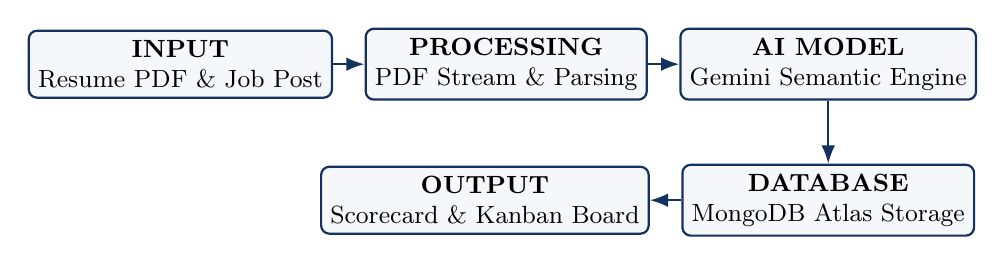
\begin{tikzpicture}[
    node distance=0.8cm and 0.4cm,
    every node/.style={font=\small},
    block/.style={rectangle, draw=primary, fill=lightgray, thick, rounded corners=3pt, minimum width=2.8cm, minimum height=0.85cm, align=center},
    arrow/.style={-Latex, thick, primary}
]
    \node (input) [block] {\textbf{INPUT}\\Resume PDF \& Job Post};
    \node (proc) [block, right=of input] {\textbf{PROCESSING}\\PDF Stream \& Parsing};
    \node (model) [block, right=of proc] {\textbf{AI MODEL}\\Gemini Semantic Engine};
    \node (db) [block, below=of model] {\textbf{DATABASE}\\MongoDB Atlas Storage};
    \node (output) [block, left=of db] {\textbf{OUTPUT}\\Scorecard \& Kanban Board};

    \draw [arrow] (input) -- (proc);
    \draw [arrow] (proc) -- (model);
    \draw [arrow] (model) -- (db);
    \draw [arrow] (db) -- (output);
\end{tikzpicture}
\vspace{0.3cm}

\raggedright
\textbf{Step-by-Step Execution Stages:}
\begin{enumerate}[label=\textbf{Step \arabic*:}, leftmargin=1.8em, itemsep=2pt]
    \item \textbf{Input Stage:} A candidate submits their resume in PDF format; recruiters submit structured role criteria.
    \item \textbf{Processing Stage:} \texttt{multer} buffers the upload in-memory, and \texttt{pdf-parse} extracts raw text content, sanitizing and normalizing whitespace.
    \item \textbf{Entity Extraction \& Semantic Reasoning:} Google Gemini processes the resume text against the target job description to assess core skills, adjacent technologies, and domain experience.
    \item \textbf{Database Persistence:} Evaluation results, applicant states, and user sessions are stored securely in MongoDB Atlas.
    \item \textbf{Output Stage:} The candidate views their diagnostic score, matched skills, and gap report. Simultaneously, the recruiter's Kanban board updates with auto-ranked candidate profiles.
\end{enumerate}

\newpage

% ==========================================
% 9. TECHNOLOGIES USED
% ==========================================
\section{Technologies Used}
The technologies utilized across all layers of the Aptly.AI architecture are outlined below:

\vspace{0.2cm}
\begin{center}
\renewcommand{\arraystretch}{1.18}
\begin{tabularx}{\textwidth}{l p{5.2cm} X}
\toprule
\textbf{\color{primary}Category} & \textbf{\color{primary}Technology} & \textbf{\color{primary}Role in Project} \\
\midrule
\textbf{Programming Language} & JavaScript (ES6+), Node.js (v20+) & Full-stack development and server execution \\
\textbf{Frontend} & React.js (v18), Vite, Vanilla CSS & Responsive SPA, paper-card UI, and state routing \\
\textbf{Backend} & Node.js, Express.js (v5) & RESTful API endpoints and middleware architecture \\
\textbf{Database} & MongoDB Atlas, Mongoose (v9) & Cloud document database for users, jobs, applications \\
\textbf{Machine Learning / AI} & Google Gemini API (\texttt{@google/genai}) & Semantic resume scoring, gap analysis, and chatbot \\
\textbf{File Parsing} & \texttt{pdf-parse}, \texttt{multer} & Buffer stream extraction for PDF resume documents \\
\textbf{Security} & JWT, \texttt{bcryptjs}, Helmet, Rate-Limit & Token auth, password encryption, rate limiting \\
\textbf{IDE} & VS Code / Google Antigravity & Development environment and terminal workflows \\
\textbf{Version Control} & Git / GitHub & Source code tracking and team collaboration \\
\bottomrule
\end{tabularx}
\end{center}

\vspace{0.3cm}

% ==========================================
% 10. MODULES
% ==========================================
\section{Modules}
The Aptly.AI architecture is organized into five core functional modules:

\begin{enumerate}[label=\textbf{Module \arabic* --}, leftmargin=2em, itemsep=5pt]
    \item \textbf{Authentication and User Management:}
    Secures user onboarding and access. Provides role-based registration and login for both Candidates and Recruiters using password hashing (\texttt{bcryptjs}) and stateless JSON Web Tokens (JWT). Client-side routes are guarded by protected wrappers.

    \item \textbf{Data and Document Management:}
    Handles ingestion and validation of job listings and resume documents. Implements stream-based PDF parsing via \texttt{multer} and \texttt{pdf-parse} to extract text without local file storage risks, saving structured records to MongoDB Atlas.

    \item \textbf{Main Processing and Semantic Scoring Engine:}
    Replaces rudimentary keyword searches with multi-vector semantic evaluation. Assesses candidates based on direct technical skills, adjacent frameworks, and production experience. Delivers a deterministic 0--100\% match score with structured feedback.

    \item \textbf{Job Quality and Bias Analysis:}
    Evaluates recruiter job descriptions in real time. Analyzes readability, clarity, and requirement specificity, while actively flagging exclusionary or biased language to promote fair and inclusive hiring.

    \item \textbf{Reports and Recruiter Kanban Dashboard:}
    Generates actionable visual outcomes. Delivers detailed diagnostic scorecards with skill-gap breakdowns for applicants, and powers an interactive, drag-and-drop-style Kanban pipeline with dynamic threshold filtering for recruiters.
\end{enumerate}

\newpage

% ==========================================
% 11. EXPECTED OUTCOME
% ==========================================
\section{Expected Outcome}
The completed Aptly.AI system achieves the following key outcomes:
\begin{itemize}[leftmargin=1.5em, itemsep=2.5pt]
    \item \textbf{Elimination of Keyword Rejection Errors:} Qualified developers with relevant, adjacent technical experience are no longer discarded due to slight phrasing differences.
    \item \textbf{Sub-Second Resume Screening:} Reduces candidate evaluation turnaround from several days to under 1.5 seconds per applicant.
    \item \textbf{Transparent Candidate Experience:} Replaces black-box rejection emails with actionable diagnostic scorecards that highlight exactly which skills candidates should learn.
    \item \textbf{Efficient Recruiter Workflows:} Enables recruiters to instantly identify top-tier talent via automated candidate ranking and dynamic Kanban staging.
    \item \textbf{Higher Job Description Quality:} Encourages clear, inclusive job postings that attract diverse, highly qualified candidate pools.
\end{itemize}

% ==========================================
% 12. FUTURE SCOPE
% ==========================================
\section{Future Scope}
To expand upon the current foundation, the following enhancements are planned:
\begin{itemize}[leftmargin=1.5em, itemsep=2.5pt]
    \item \textbf{Mobile Application:} Develop a cross-platform React Native mobile app for on-the-go candidate status notifications and recruiter applicant triage.
    \item \textbf{Cloud Deployment \& Microservices:} Containerize core services using Docker and orchestrate on Kubernetes for elastic auto-scaling during high-volume campus hiring drives.
    \item \textbf{Advanced Analytics:} Implement interactive comparative skill-gap radar charts and multi-candidate benchmark matrices.
    \item \textbf{AI-Based Recommendations:} Deliver personalized learning roadmap suggestions to candidates based on identified competency gaps.
    \item \textbf{Automated Notifications \& Scheduling:} Integrate Google Calendar and Calendly APIs to automate technical interview scheduling upon applicant shortlisting.
    \item \textbf{Integration with External APIs:} Directly sync job posts and candidate profiles with LinkedIn, GitHub, and corporate HRMS platforms.
    \item \textbf{Improved Security and Scalability:} Introduce automated anti-cheat PDF heuristic detection and enterprise single-sign-on (SSO) authentication.
\end{itemize}

% ==========================================
% 13. REFERENCES
% ==========================================
\section{References}
\begin{enumerate}[label={[\arabic*]}, leftmargin=2em, itemsep=2.5pt]
    \item Google DeepMind: \textit{Gemini API Structured Outputs and Multimodal Reasoning Specification}, 2025--2026. URL: \url{https://ai.google.dev/}
    \item React Team: \textit{React 18 and Vite Single Page Application Architecture Guidelines}, 2025. URL: \url{https://react.dev/}
    \item MongoDB Inc.: \textit{Mongoose Object Data Modeling (ODM) Best Practices}, 2025. URL: \url{https://mongoosejs.com/}
    \item A. Vasiliev et al.: \textit{``Semantic Natural Language Processing in Automated Applicant Tracking Systems,''} IEEE Transactions on Emerging Technologies, 2024.
    \item Express.js Team: \textit{Express v5 RESTful Routing, Middleware, and Security Architecture}, 2025. URL: \url{https://expressjs.com/}
    \item Aptly.AI Live Production Platform: \url{https://aptly-zeta.vercel.app/}
\end{enumerate}

\vspace{0.4cm}

% ==========================================
% FINAL SYNOPSIS CHECKLIST
% ==========================================
\subsection*{Final Synopsis Checklist}
\begin{itemize}[label=$\square$, leftmargin=2em, itemsep=2pt]
    \item Cover Page (Project Details, Student Credentials, Guide Name, Institution)
    \item Project Title (Official Assigned Code: P\_204 and Title)
    \item Introduction (Domain Background and Relevance)
    \item Problem Statement (Specific Inefficiencies in Current Systems)
    \item Objectives (Clear, Measurable Project Goals)
    \item Proposed Solution (Candidate, Recruiter, and AI Copilot Workflows)
    \item Scope of the Project (In Scope vs. Out of Scope)
    \item Methodology / Working (Pipeline Architecture and Execution Stages)
    \item Technologies Used (Structured Categorical Matrix)
    \item Modules (Five Core System Modules Defined)
    \item Expected Outcome (Measurable Performance and Impact Metrics)
    \item Future Scope (Key Planned Advancements)
    \item References (Academic Papers and Official Documentation)
\end{itemize}

\end{document}
